\documentclass[11pt,a4paper,dvipsnames,twosided,final]{article}

\usepackage[deliverable]{IOHKCoverPage}

% data for Deliverable header -- added by KH from an EU H2020 project template
\DeliverableNumber{SL-D4}
\DeliverableTitle{An Introduction to the Shelley Incentives Scheme}{Incentives Scheme Intro.}
\DeliverableResponsible{Formal Methods Team}
\EditorName{Kevin Hammond, \IOHK}
\Authors{Kevin Hammond \quad \texttt{<kevin.hammond@iohk.io>}
}
\DueDate{14$^{\textrm{th}}$ October 2019}
\SubmissionDate{14$^{\textrm{th}}$ October 2019}{2019/10/14}
\LeaderName{Philipp Kant, \IOHK}
\InstitutionAddress{\IOHK}
\Version{0.2}
\Project{Shelley Ledger}
\DisseminationDR

\usepackage[margin=2.5cm]{geometry}
\usepackage{lscape}
\usepackage{iohk}
\usepackage{microtype}
\usepackage{mathpazo} % nice fonts
\usepackage{amsmath}
\usepackage{amssymb}
\usepackage{amsthm}
\usepackage{latexsym}
\usepackage{mathtools}
\usepackage{stmaryrd}
\usepackage{extarrows}
\usepackage{slashed}
%\usepackage[colon]{natbib}
\usepackage[unicode=true,pdftex,pdfa,colorlinks=true]{hyperref}
\usepackage{xcolor}
\usepackage[capitalise,noabbrev,nameinlink]{cleveref}
\usepackage{float}
%\floatstyle{boxed}
\restylefloat{figure}
\usepackage{tikz}
\usepackage{booktabs}
\usepackage{enumerate}

%% Commenting -- KH
\usepackage[obeyFinal]{todonotes}
\newcommand{\khcomment}[1]{\todo[color=blue!20]{KH: #1}}

\newcommand{\ada}{ADA{}}
\newcommand{\ADA}[1]{\textbf{\emph{\ada~{#1}}}}
\newcommand{\cardano}[1]{Cardano}

%% In-para enumeration -- KH
\usepackage{paralist}

\usepackage{caption}

\begin{document}

\hypersetup{
  pdftitle={},
  breaklinks=true,
  bookmarks=true,
  colorlinks=false,
  linkcolor={blue},
  citecolor={blue},
  urlcolor={blue},
  linkbordercolor={white},
  citebordercolor={white},
  urlbordercolor={white}
}

  \cleardoublepage%
  \tableofcontents%
  \listoffigures%
  \clearpage%

  \begin{changelog}
        \change{2019/10/09}{Kevin Hammond}{FM (\IOHK)}{Initial Version.}
        \change{2019/10/14}{Kevin Hammond}{FM (\IOHK)}{Polished slightly.}
      \end{changelog}
      \clearpage%
\begin{landscape}
\floatstyle{plain}
\restylefloat{figure}
\begin{figure*}
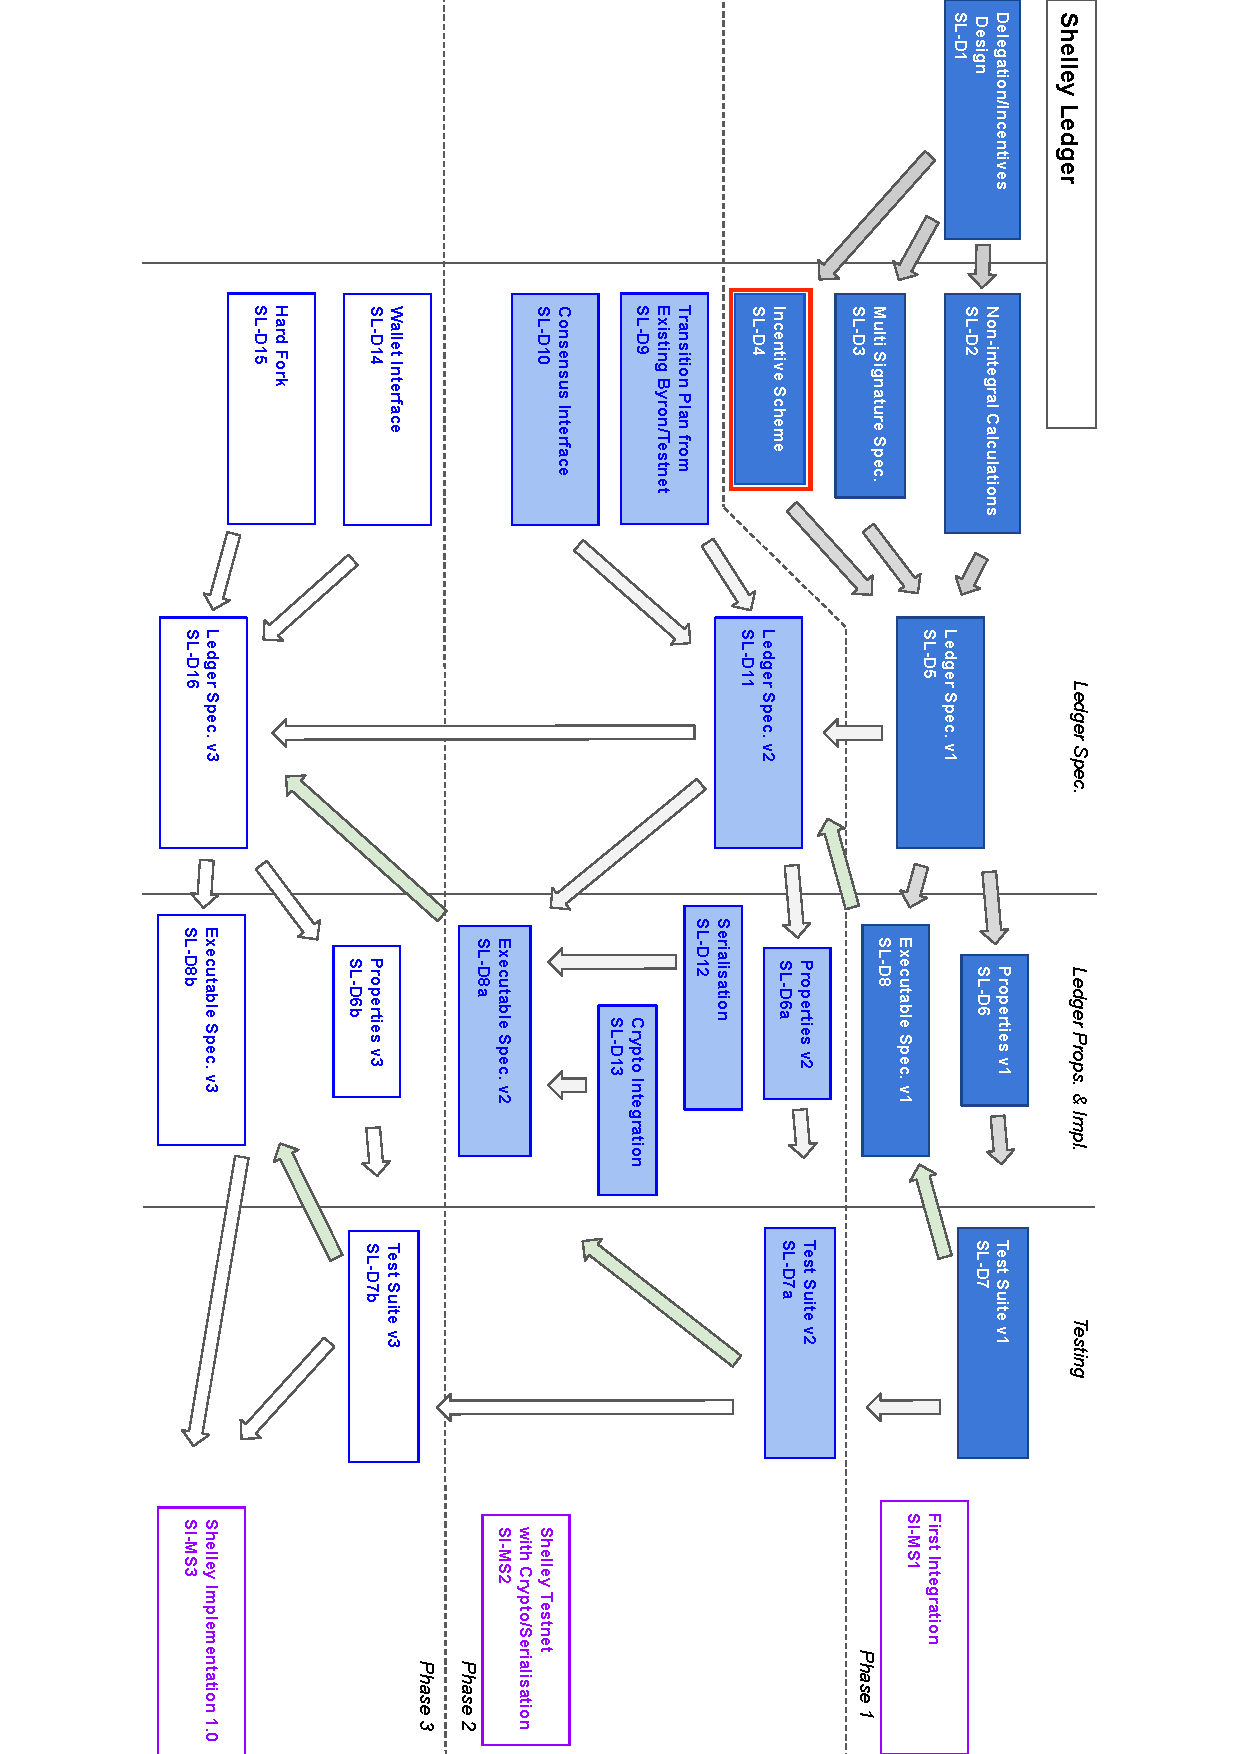
\includegraphics[scale=0.8,angle=90]{d4-depends.pdf}
\caption{Positioning of this Deliverable (outlined in red).}
\end{figure*}
\end{landscape}
%\floatstyle{boxed}
\restylefloat{figure}
\cleardoublepage
% \begin{center}
% \large{Executive Summary}
% \end{center}

% \cleardoublepage
\renewcommand{\thepage}{\arabic{page}}
\setcounter{page}{1}

\title{An Introduction to the Shelley Incentives Scheme}

\author{Kevin Hammond  \\ {\small \texttt{kevin.hammond@iohk.io}}}

\maketitle

\begin{abstract}
  \noindent
  This document provides a high-level overview of the proposed incentives rewards schemes for
  the Shelley incentived Testnet and the subseqent Mainnet, highlighting key
  differences between the two schemes.  It is intended to act as a
  simple, easy to follow, guide to the operation of each of the incentives schemes.
  It assumes a basic familiarity with the concepts of a \emph{blockchain} approach.
  The incentives scheme is designed to ensure the correct operation of the Ouroborous Praos
  protocol, including maintaining built-in defences against ``Sybil-in-Sybil'' security attacks
  that could lead to corruption of the blockchain.
  A simplified version of the incentives scheme is used for the Incentivised Testnet, using fixed rewards,
  omitting fee calculations, influence and apparent performance etc. (some of these features may be
  added in later versions of the Incentivised Testnet).
  This document is based on SL-D1 (Delegation/Incentives Design)~\cite{delegation_design} and feeds in to SL-D5
  (Formal Ledger Specification. Version 1)~\cite{shelley_spec} as well as the online rewards calculator and the Shelley Incentivised Testnet and Mainnet  implementations and quality assurance programmes.
\end{abstract}

\clearpage
\section{Introduction}
\label{sec:introduction}

Figure~\ref{fig:terminology} gives some basic terminology.
The Shelley implementation rewards those \ada{} holders who either own active stake pools
(\emph{Owners}) or who delegate stake to active stake pools (\emph{Delegators}).
In line with the design of the Ouroborous protocol~\cite{ouroboros_classic}, the Stakepool receives
rewards in proportion to the stake that it \emph{controls} (``proof of
stake'') rather than in proportion to the work that it does (``proof of work'').
This has cost, efficiency and safety advantages.
The level of rewards that the implementation provides is designed to help ensure that no single entity can
dominate the system by \emph{controlling} excessive amounts of \ada{}.  This is achieved by creating intrinsic
balancing mechanisms that will naturally spread all the active stake among a large number of stakepools.
In particular, the rewards to any one \emph{Stakepool} may be capped to a pre-determined limit,
meaning that both delegators and owners will receive less reward if too much stake is controlled by a single stakepool,
so encouraging the creation of additional, smaller stakepools.
% This includes limiting the amount of \ada{} that is delegated to any one \emph{stakepool}.
The overall theory that ensures this is described in the Ouroborous Praos research
paper~\cite{ouroboros_praos}. The design of the incentives and delegation scheme is described
in~\cite{delegation_design}.

\textbf{\emph{Note: this document is subject to change.  In particular, it may be necessary to include a simplified fees calculation
  in the incentivised testnet, where the fees are given to the treasury\khcomment{Check fees.}.}}

\begin{figure}[t]
  \begin{center}
\begin{tabular}{||l|p{12cm}||}
  \hline \hline
\textbf{Term} & \textbf{Definition} \\\hline
  Stakepool & A system that is actively participating in the creation of blocks on the \cardano{} blockchain  \\\hline
  Stake & An amount of \ada{} that is \emph{controlled} by a Stakepool.\\\hline
  Epoch & A fixed period of time during which blocks are created.\\\hline
Operator & The entity that is responsible for running a Stakepool. \\\hline
Owner(s) & The entities that \emph{pledge} stake to the Stakepool. \\\hline
  Delegator(s) & The entities that \emph{delegate} stake to the Stakepool.\\\hline
  Treasury & Central Repository of \ada.\\\hline
  Reserve & \ada{} that is not yet in circulation.\\\hline
  Reward & \ada{} that is given to a performant Stakepool.\\\hline
  \hline
\end{tabular}
\end{center}
\caption{General Terminology}
\label{fig:terminology}
\end{figure}

\newpage
\subsection{General Parameters}

\begin{figure}[h!]
\begin{center}
\begin{tabular}{||l|l|p{10cm}|l||}
  \hline \hline
\textbf{Parameter} & \textbf{Expected Value} & \textbf{Definition} \\\hline
\emph{k} & 50-1000 & The Target Number of Stakepools \\\hline
$T$ & 10\% & The Treasury Top Slice Percentage \\\hline
$MER$ & 10\% &  The ``Monetary Expansion Rate'' per Year \\\hline
$E$ & 1-5 &  Elapsed days per \cardano{} Epoch \\\hline
  \hline
\end{tabular}
\end{center}
\caption{Key Operational Parameters.}
\end{figure}

\noindent
Four key operating parameters are set by the community (the initial values will be determined by \IOHK):
$k$, the target number of stakepools;
$T$, the treasury top slice percentage;
$MER$, the monetary expansion per year;
and
$E$, the length of each epoch, in days.
%
The target number of Stakepools is used to cap the rewards that any individual stakepool can receive. The intention is to encourage the creation of more stakepools, and to avoid domination by any single stake holder.
The \emph{treasury top slice percentage} is the fraction of reward that is allocated to the treasury to cover fixed operating costs, and
ensure the long-term viability both of the \cardano{} system and of \ada{} as a currency.  It is initially set to a small percentage (10\%) of the rewards.
The \emph{monetary expansion rate} is the rate at which rewards are allocated from the \emph{reserves} of \ada{}.

\begin{figure}[h!]
\begin{center}
\begin{tabular}{||l|l|p{6cm}|l||}
  \hline \hline
\textbf{Parameter} & \textbf{Value} & \textbf{Description} & \textbf{Calculated as} \\\hline
${Ada}_{Tot}$ & \ADA{45bn} & The total \ada{} that could ever be created & \\\hline
\emph{P} & 20\%-50\% & Participation Rate in the Shelley Incentivised Testnet & \\\hline
${Ada}_{circ}$ & \ADA{31bn} & The total \ada{} in circulation at Shelley launch & \\\hline
${Ada}_{rsv}$ & \ADA{14bn} & The total \ada{} in the reserves at Shelley launch & ${Ada}_{Tot} - {Ada}_{circ}$ \\\hline
\hline
\end{tabular}
\end{center}
\caption{Parameters that are set by External Factors (e.g. \ada{} holders).}
\end{figure}

\noindent
Several parameters are pre-determined by external factors. These include the
total \ada{} that could ever be created, ${Ada}_{Tot}$;
the total \ada{} that is in \emph{circulation} when the Shelley system launches
(i.e. all \ada{} that is held by any entity on the launch date), ${Ada}_{circ}$;
and the \ada{} that is held in reserve when the system starts.
These values are fixed and will not change.

\clearpage
\subsection{Stakepools}

\subsubsection*{Operator-Set Parameters}

\begin{figure}[h!]
\begin{center}
\begin{tabular}{||l|l|p{9cm}||}
  \hline \hline
\textbf{Parameter} & \textbf{Range} & \textbf{Description} \\\hline
{\color{red} $\textit{Pool}_{cost}$} &  & {\color{red} Cost per day in \ada{}} \\\hline
{\color{red} ${Pool}_{margin}$} &  {\color{red} 0\%-100\%} & {\color{red} Percentage fee on rewards (the ``margin'')} \\\hline
  \hline
\end{tabular}
\end{center}
\caption{Key Parameters that are set by the StakePool Operator.}
\end{figure}

\noindent
The two main parameters that need to be set by the \emph{operator} are the cost per day that will be charged to
the pool (in \ada), $\textit{Pool}_{cost}$; and the percentage of any rewards that will subsequently be taken as a fee, ${Pool}_{margin}$.
The cost is subtracted from the total rewards that are earned by the pool before any rewards are distributed.
These parameters are advertised by the stakepool and used as part of the public ranking scheme.

\subsubsection*{The \ada{} that is controlled by the Stakepool}

\begin{figure}[h!]
\begin{center}
\begin{tabular}{||l|p{9cm}|l||}
  \hline \hline
\textbf{Parameter} & \textbf{Description} & \textbf{Calculated as} \\\hline
{\color{red} ${Pool}_\textit{pledge}$} & {\color{red} \ada{} that is pledged to the Stakepool by the Owner(s)} & \\\hline
{\color{blue} ${Pool}_\textit{deleg}$} & {\color{blue}  \ada{} that is delegated to the Stakepool} & \\\hline
${Pool}_{Tot}$ & All \ada{} that is controlled by the Stakepool & ${Pool}_\textit{pledge} + {Pool}_\textit{deleg}$ \\\hline
${Pool}_\%$ & Fraction of the \ada{} in circulation that is controlled by the Stakepool & {\large $\frac{{Pool}_{Tot}}{{Ada}_{circ}}$} \\\hline
  \hline
\end{tabular}
\end{center}
\caption{The \ada{} that is controlled by a StakePool.}
\end{figure}

\noindent
The rewards that are received by the Stakepool will be proportional to the amount of \ada{} that it controls.
This is calculated as the sum of the \ada{} that is \emph{pledged} to the Stakepool by the owners(s) plus
the additional \ada{} that is \emph{delegated} to the Stakepool.  An owner may \emph{delegate} to a Stakepool if
they wish as well as \emph{pledging} to it, but would receive lower rewards.  In return for receiving
higher rewards, \emph{pledging} incurs higher risk, requiring owners to \emph{trust} each other.


\clearpage
\section{The Simplified Incentives Scheme (Shelley Incentived Testnet)}
\label{sec:testnet}

The simplified scheme calculates rewards based on the total number of blocks that each stake pool produces,
and distributes a fixed amount of \ada{} per epoch.
Since \cardano{} is based on \emph{proof of stake}, then on average, each stake pool will produce
rewards that are proportional to the stake that it holds.  So, if e.g. a pool holds 1\% of the total
\ada{} in circulation, then it will receive, on average, 1\% of the total rewards that are allocated to all the
stakepools.

\begin{figure}[h!]
\begin{center}
\begin{tabular}{||l|l|p{6cm}|l||}
  \hline \hline
\textbf{Parameter} & \textbf{Expected Value} & \textbf{Description} & \textbf{Calculated as} \\\hline
\emph{P} & 20\%-50\% & Participation Rate in the Testnet & \\\hline
${Ada}_{tnet}$ & \ADA{15.5bn} @ $P=50\%$ & The \ada{} circulating in the Testnet & $P \times {Ada}_{circ}$ \\\hline
  \hline
\end{tabular}
\end{center}
\caption{\ada{} in Circulation in the Incentivised Testnet.}
\end{figure}

\noindent
The total \ada{} that is circulating in the Testnet is derived from the \emph{participation rate} (the percentage of the total \ada{} in
circulation that is available to be staked in the Incentivised Testnet). This will be determined at the date when the
Testnet launches and will then remain fixed\khcomment{Check - no \ada{} can be transferred later -
affects the calculations/reward?}.  It is assumed that this is likely to be 20\%-50\% of the total \ada{} in
circulation.


\begin{figure}[h!]
\begin{center}
\begin{tabular}{||l|l|p{6cm}|l||}
  \hline \hline
\textbf{Parameter} & \textbf{Expected Value} & \textbf{Description} & \textbf{Calculated as} \\\hline
\emph{E} & 1 & Days per Epoch in the Testnet & \\\hline
${Distr}_E$ & \ADA{3.84M} & Distribution per Epoch in the Testnet & $\frac{\large {Ada}_{rsv} \times \textit{MER}}{\large 365 \div E}$ \\\hline
$T_E$ & \ADA{384K} & Treasury Top Slice per Day & $R_E \times T$ \\\hline
$R_E$ & \ADA{3.45M} & Total Rewards per Epoch & ${Distr}_E - T_E$ \\\hline
  \hline
\end{tabular}
\end{center}
\caption{Total Distribution and Rewards per Epoch.}
\label{fig:distrib}
\end{figure}

\noindent
The total \ada{} that is distributed per epoch in the Incentivised Testnet (${Distr}_E$) is calculated from the initial
value of the \ada{} reserves, ${Ada}_{rsv}$, and the fixed monetary expansion rate, \textit{MER}.
An equal distribution is given per epoch.  The top slice that is allocated to the treasury ($T_E$) is
deducted from this distribution, and the remainder is then allocated to the Stakepools as rewards ($R_E$).
For simplicity, in the Incentivised Testnet, the length of each epoch has been set to 1 day.

\clearpage
\subsection{The Rewards that are received by a Stakepool}

\begin{figure}[h!]
\begin{center}
\begin{tabular}{||l|l|p{6cm}|l||}
  \hline \hline
\textbf{Parameter} & \textbf{Expected Value} & \textbf{Definition} & \textbf{Calculated as} \\\hline
{\color{red} ${Pool}_\textit{pledge}$} & & {\color{red} \ada{} that is pledged to the Stakepool by the Owner(s)} & \\\hline
{\color{blue} ${Pool}_\textit{deleg}$} & & {\color{blue} \ada{} that is delegated to the Stakepool} & \\\hline
${Pool}_{Tot}$ & & All \ada{} that is controlled by the Stakepool & ${Pool}_\textit{pledge} + {Pool}_\textit{deleg}$ \\\hline
  ${Pool}_\%$ & & Fraction of the \ada{} in circulation that is controlled by the Stakepool & {\large $\frac{{Pool}_{Tot}}{{Ada}_{tnet}}$} \\\hline
&&&  \\\hline
$R_E$ & \ADA{3.45M} & Total Rewards per Epoch & ${Distr}_E - T_E$ \\\hline
&&&  \\\hline
{\color{red} $\textit{Pool}_{cost}$} &  & {\color{red} Cost per day in \ada{}} & \\\hline
{\color{red} ${Pool}_{margin}$} &  {\color{red} 0\%-100\%} & {\color{red} Percentage fee on rewards (the ``margin'')} & \\\hline
\emph{N} & & The Number of Blocks that were allocated to the StakePool & \\\hline
\emph{n} & & The Number of Blocks actually Produced by the Stakepool & \\\hline
\emph{k} & 50-1000 & The Target Number of Stakepools & \\\hline
\emph{z} & 0.001-0.02 & The Rewards Limit Fraction & $\frac{1}{k}$ \\\hline
\hline
\end{tabular}
\end{center}
\caption{Parameters Governing the Rewards to a Stakepool.}
\label{fig:rewards}
\end{figure}

\noindent
The parameters governing the Stakepool reward calculation are shown above.  The only new
parameters are $n$, $N$ and $z$. $n$ and $N$ are measured by the system; $z$ is calculated from the
target number of StakePools, $k$.  These parameters limit the rewards that can be received by any Stakepool.
\khcomment{Check that ${Ada}_{tnet}$ is a fixed value.}

\begin{figure}[h!]
\begin{center}
\begin{tabular}{||l|p{6cm}|l||}
  \hline \hline
\textbf{Parameter}  & \textbf{Definition} & \textbf{Calculated as} \\\hline
$R_{Gross}'$ & The Average Gross Reward to the StakePool & $R_E \times \textrm{min} (z,{Pool}_\%)$ \\\hline
$R_{Gross}$ & The Actual Gross Reward to the StakePool & $R_{Gross}' \times \textrm{min} (100\%,\frac{n}{N})$ \\\hline
${Pool}_{costE}$ & Pool Operator Costs for the Epoch & $\textrm{min}(\textit{Pool}_{cost} \times E,R_{Gross})$ \\\hline
$R_{Net}$  & The Net Reward to the StakePool & $R_{Gross} - {Pool}_{costE}$ \\\hline
$R_{Owner}$ & The Total Reward to the Owner(s) & $R_{Net} \times {Pool}_{margin} $ \\\hline
$R_{Deleg}$ & The Total Reward to the Delegators & $R_{Net} - R_{Owner}$ \\\hline
$\textit{Income}$ & The Total Pool Owner Income & ${Pool}_{costE} + R_{Owner}$ \\\hline
\hline
\end{tabular}
\end{center}
\caption{Calculation of the Total Stake Pool Reward.}
\end{figure}

\noindent
The gross reward that is received by the Stakepool is, on average, directly proportional to the
stake that it controls, as a proportion of the total \ada{} that is in circulaton.
It is limited by the rewards limit fraction, and reduced in proportion to the ratio of blocks it produced
to blocks it was allocated (the ``performance'' of the StakePool) to give $R_{Gross}$.
Once the pool operator costs are subtracted,
the net reward is then distributed to the owner(s) and delegators in proportion to the
stake that each group controls.  The total pool income is then the sum of the operator costs and the pool owner rewards.
Note that if there is insufficient gross reward to cover the operator costs, all the reward will be accrued to those
costs, leaving no further reward to be distributed to the owners or delegators.

\subsubsection*{The Rewards that are received by each Delegator}

\begin{figure}[h!]
\begin{center}
\begin{tabular}{||l|p{6cm}|l||}
  \hline \hline
\textbf{Parameter} & \textbf{Definition} & \textbf{Calculated as} \\\hline
${Pool}_{Tot}$ & All \ada{} that is controlled by the Stakepool & ${Pool}_\textit{pledge} + {Pool}_\textit{deleg}$ \\\hline
$R_{Deleg}$ & The Total Reward to the Delegators & $R_{Net} - R_\textit{Owner}$ \\\hline
$D_{Stake}$ & The \ada{} that is delegated by Delegator $D$ & \\\hline
$D_\%$ & The proportion of \ada{} in the pool that is delegated by $D$ & \\\hline
$D_{Rewards}$ & The \ada{} rewards that are received by $D$ & $R_{Net} \times R_\textit{Owner}$ \\\hline
\hline
\end{tabular}
\end{center}
\caption{The Rewards that are received by a specific Delegator, $D$.}
\end{figure}

\noindent
The rewards that are received by an individual delegator are directly proportional to the
stake that that delegator has placed in the Stakepool, calculated from the net rewards to the
Stakepool.

\subsubsection*{The Rewards that are received by each StakePool Owner}

\begin{figure}[h!]
\begin{center}
\begin{tabular}{||l|p{6cm}|l||}
  \hline \hline
\textbf{Parameter}  & \textbf{Definition} & \textbf{Calculated as} \\\hline
$R_\textit{Owner}$ & The Total Reward to the Owner(s) & $R_{Net} \times {Pool}_{margin} $ \\\hline
$n_\textit{Owner}$ & The number of Owners & \\\hline
$O_{Rewards}$ & The \ada{} rewards that are received by each owner & $R_\textit{Owner} \div n_\textit{Owner}$ \\\hline
\hline
\end{tabular}
\end{center}
\caption{The Rewards that are received by each Owner.}
\end{figure}

\noindent
In the Incentivised Testnet, the owner rewards are divided equally among the
owners, regardless of the proportion of stake that they pledge.  The assumption
is that, in practice, each owner will pledge an equal amount of stake, but this
is not enforced by the \cardano{} system.

\clearpage
\subsection{Calculating Rewards in External Currencies}

\begin{figure}[h!]
\begin{center}
\begin{tabular}{||l|p{6cm}|l||}
  \hline \hline
\textbf{Value} & \textbf{Description} & \textbf{Calculated as} \\\hline
$R_A$ &  Rewards value in \ada{} &\\\hline
$ER_D$ &  Dollar Price per \ada{} &\\\hline
$R_D$ &  Rewards value in dollars & $R_A \times ER_D$ \\\hline
\hline
\end{tabular}
\end{center}
\caption{Calculating Monetary Rewards}
\label{fig:monetary}
\end{figure}

\noindent
As usual, rewards in \ada{} can easily be converted to an external dollar or other currency equivalent using
the current exchange rate, $ER_D$, as shown % in Figure~\ref{fig:monetary}
above.  For example, if the rewards are \ADA{10,000} and the exchange rate is
\$0.04 (1 \ada{} is worth 4 cents).  Realising this value would require the use of an \emph{exchange},
of course.

\clearpage
\subsection{Worked Example}


This example is taken from the \IOHK{} internal calculator at:
\url{https://docs.google.com/spreadsheets/d/1c-KmCNBIMZjHN7wdsrNx3ac1zT8xEqodK1OyZxC_QIk/edit#gid=1365573139}

\subsubsection*{Key Parameters}
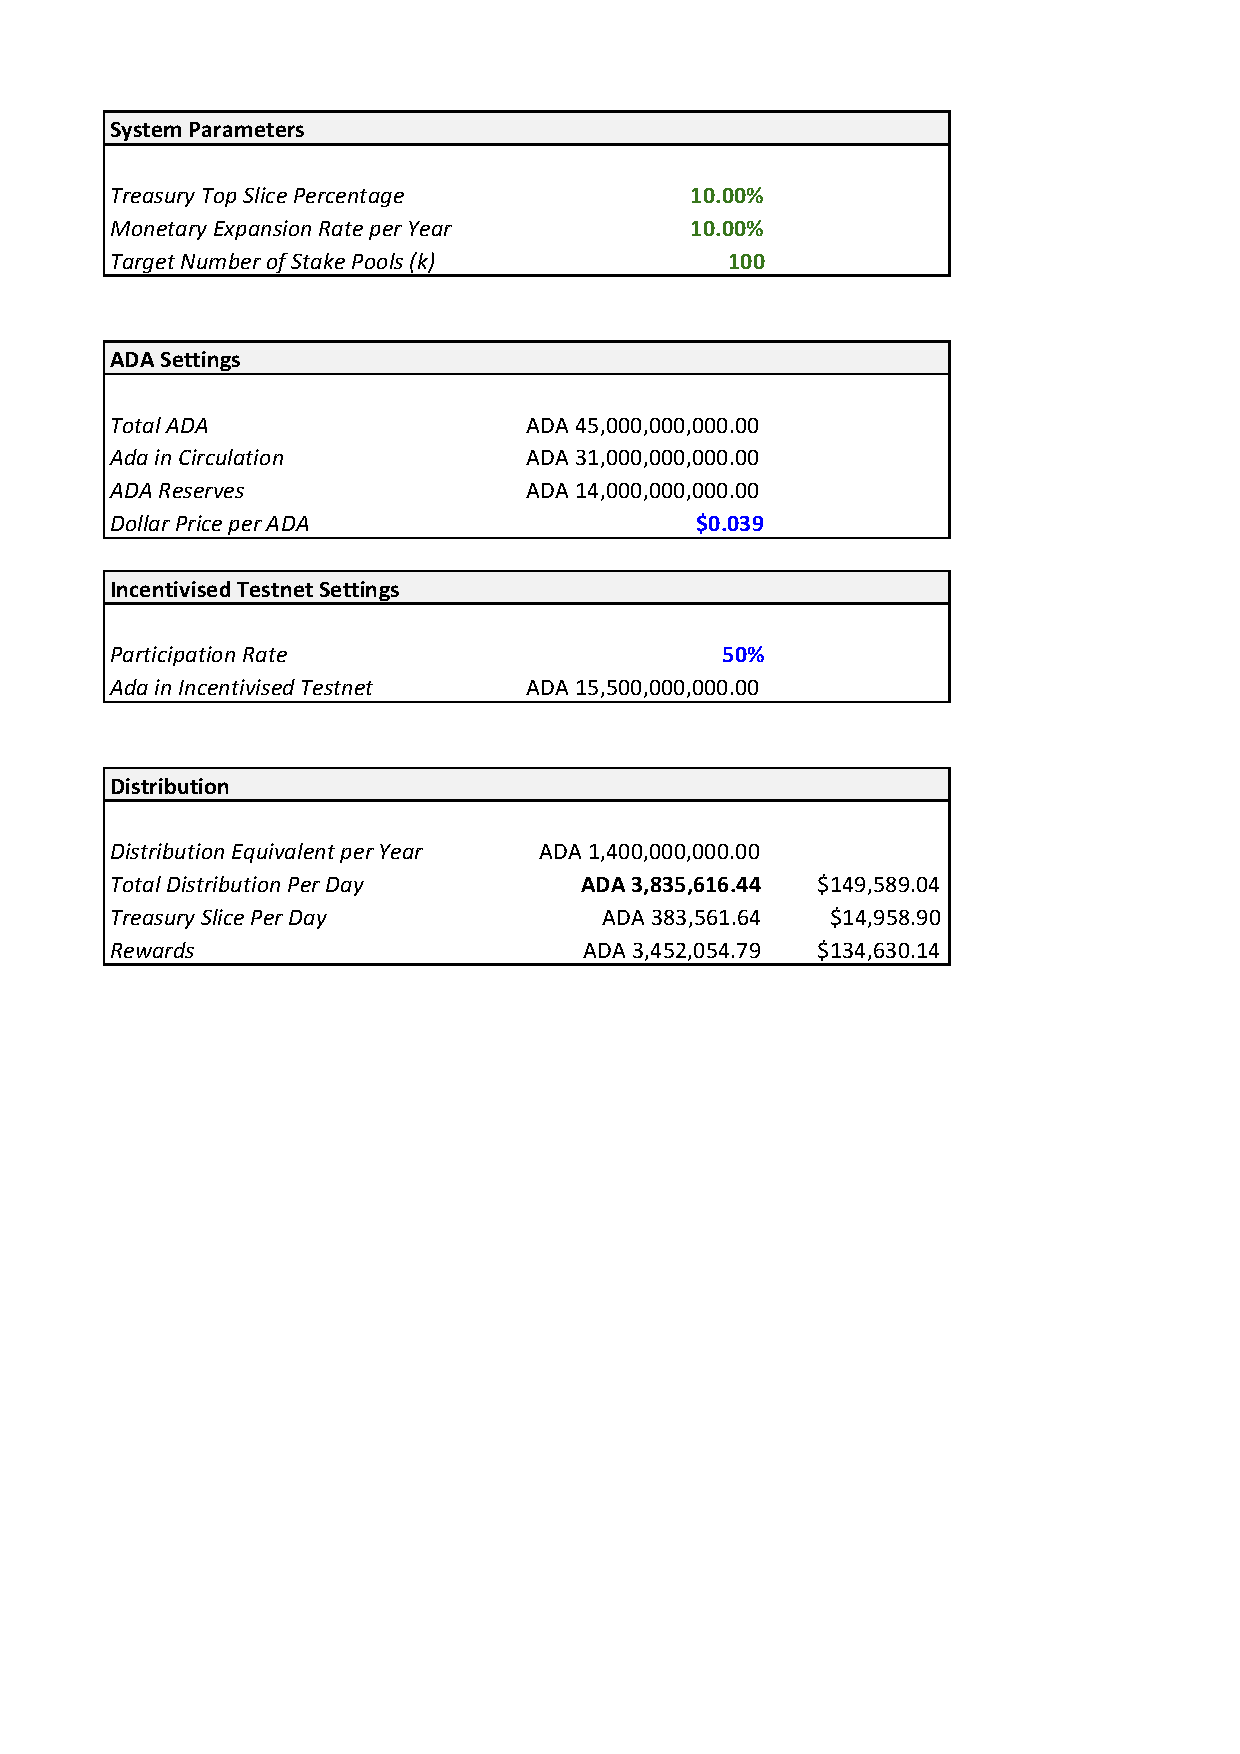
\includegraphics[height=6in]{RC1.pdf}

\noindent
This diagram shows the key parameters and settings for the rewards system, including the
rewards that are distributed from the reserves at each epoch.


\subsubsection*{Stakepool Parameters}
\includegraphics[width=\textwidth]{RC2.pdf}
\noindent
This diagram shows the Stakepool-specific parameters, including the total controlled \ada{} and the
division by owner(s) and delegators.  Here, 98.71\% of the Stakepool \ada{} is owned
by delegators.  The Stakepool receives all of its optimal rewards, since it controls
exactly the required perecentage of stake (1.00\%, corresponding to the limit set from
the $k$ parameter).

\subsubsection*{Calculated Rewards}

\hspace{-0.65in}\begin{minipage}{\textwidth}
  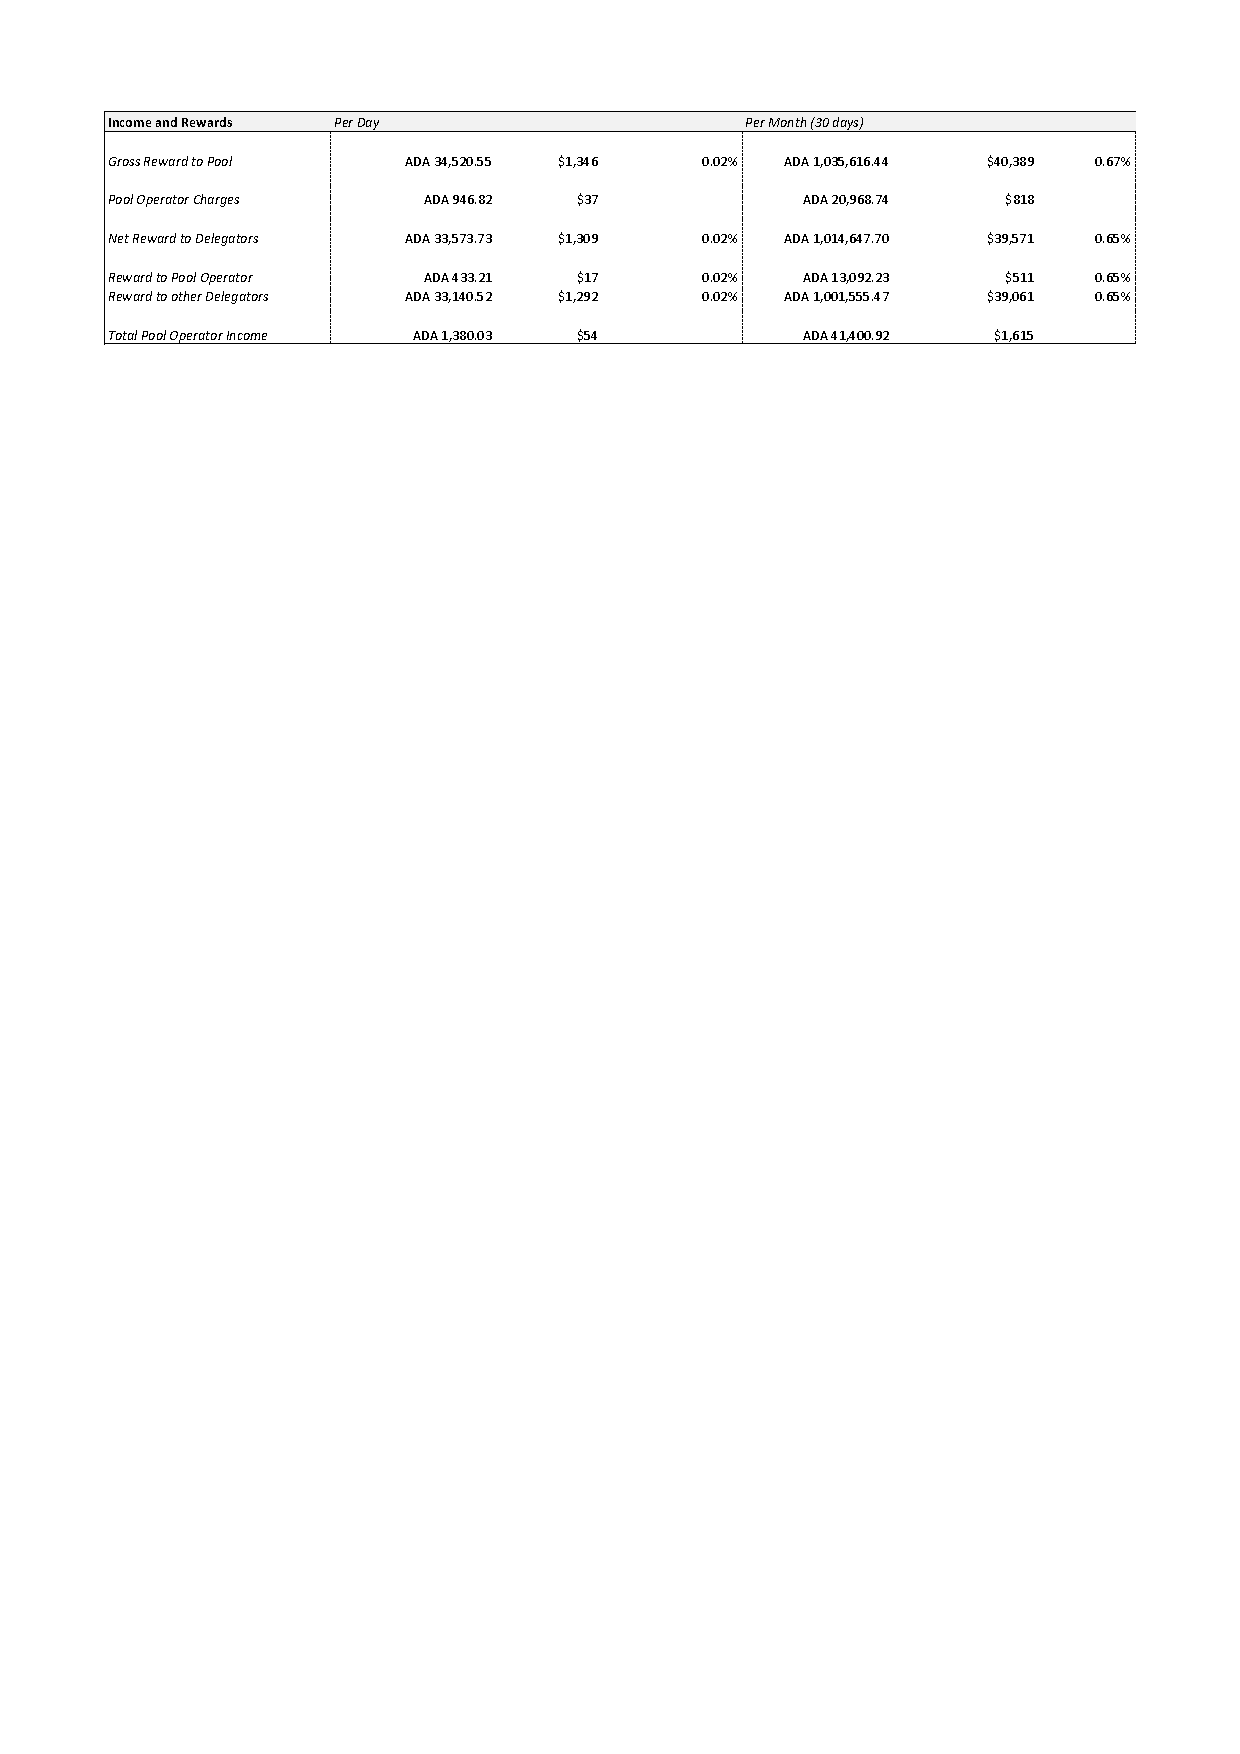
\includegraphics[width=1.2\textwidth]{RC3.pdf}
  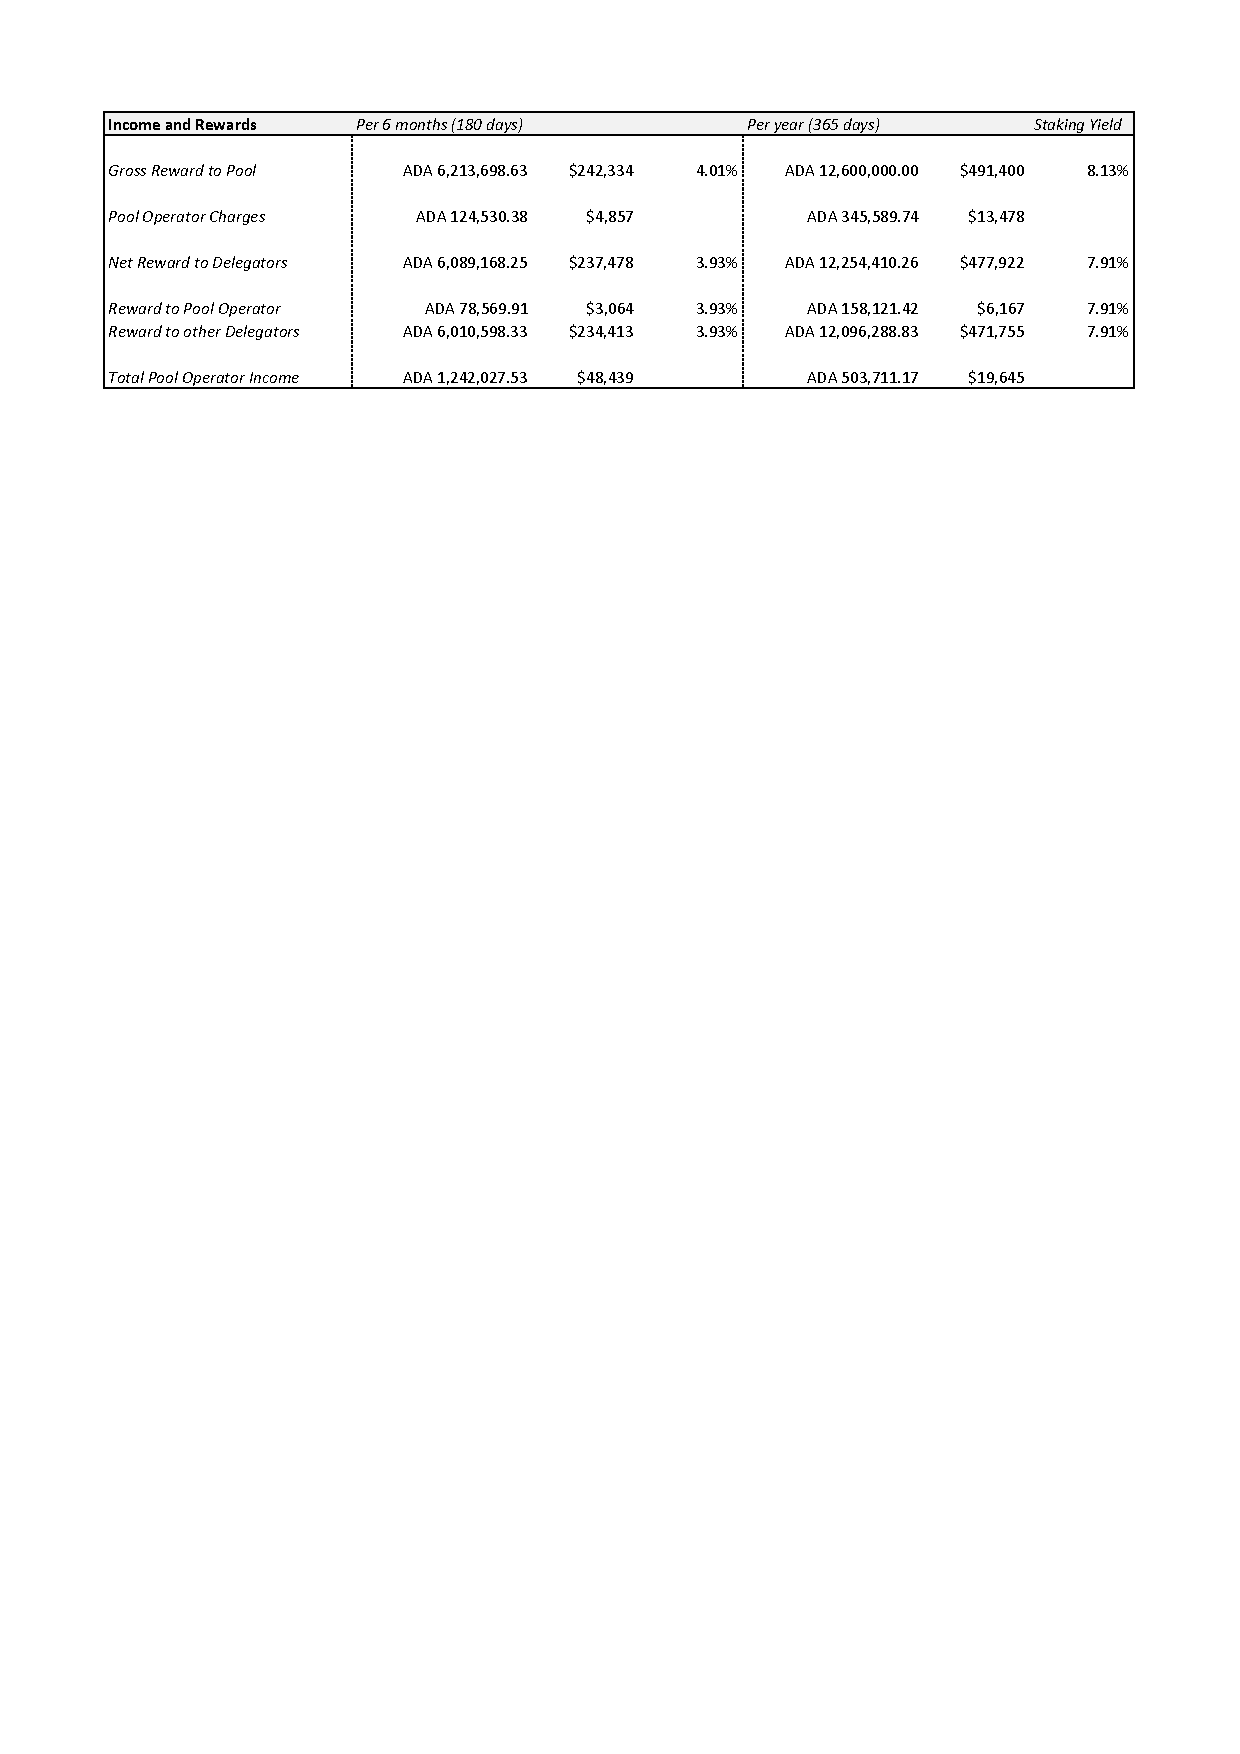
\includegraphics[width=1.2\textwidth]{RC4.pdf}
\end{minipage}

\noindent
This diagram shows the corresponding rewards that accrue to the owner(s) and delegators,
plus a calculation of the total income that is received by the owners.  We will assume that the average
and actual gross rewards are the same, i.e. if the Stakepool controls 1\% of the total \ada{} in
circulation, it will produce exactly 1\% of the blocks, that it has 100\% performance, and will therefore receive exactly 1\% of the rewards.
In total, the
owners and delegators to this Stakepool would receive a net reward that was equivalent to almost 8\% per year
(the ``staking yield'').  If there were 4 owners for the Stakepool, each would receive
25\% of the operator rewards, i.e. $\ADA{158,121.42} \div 4 ~~=~~ \ADA{39,530.36}$.
Similarly, a delegator contributing 10\% of the delegated stake would receive 10\% of
the delegator reward, i.e., $\ADA{12,096,288.83} \div 10 ~~=~~ \ADA{1,209,628.89}$.


\subsection{How rewards are returned to Owners and Delegators}

Rewards are returned through transactions using the relevant public keys, following the end
of each epoch (settlement may not be immediate, since the rewards may need to be audited).
These rewards can then be stored within a wallet, recorded on an exchange etc., as required.
In the Incentivised Testnet, however, they cannot be used for further staking.
\khcomment{Jared - do you want to check this and flesh it out if needs be?}

\clearpage
\section{The Full  Scheme as used in the Shelley Mainnet Implementation}
\label{sec:mainnet}

To be added in version 0.3 of this document.

%\clearpage
\subsection{Summary of Differences between the Two Incentives Schemes}
\label{sec:summary}

\begin{figure}[h!]
\begin{center}
\begin{tabular}{||l|p{4cm}|p{4cm}||}
  \hline\hline
  \textbf{Value} & \textbf{Incentivised Testnet} & \textbf{Mainnet}
                                              \\\hline
Treasury Top Slice Percentage
& Fixed at 10\%
& Initially set to 10\% but can be changed in future by a community vote
                                              \\\hline
Monetary Expansion Rate per Year
& fixed at 10\%
& Exponential decay from ~10\%
                                              \\\hline
 Target Number of Stake Pools
                 &
\multicolumn{2}{|p{8cm}||}{
Identical effect, the Mainnet settings will be determined based on feedback from the Testnet.
The target is expected to grow over time and may reach around 1000.
It willl initially be set low (probably 50 or 100).}
                                              \\\hline
Participation
& Any stakeholder can participate if they hold ADA as of a specific date
& Any stakeholder can participate if they hold ADA
                                              \\\hline
Fees
& None
& Included in the reward pot
                                              \\\hline
Influence Factor
& None
& Initially set to 0.1
                                              \\\hline
Pool Performance
& Not considered, except for actual block creation
& Directly affects rewards, any ``penalty'' accrues to the treasury
                                              \\\hline
Owner Rewards
& Divided equally amongst multiple owners
& Owners can decide proportions using a smart contract
                                              \\\hline
ADA that affects rewards
& any ADA that is circulating in the Testnet
& all ADA in circulation
                                              \\\hline
Stake pledged by owners
& Assumed to be fully pledged
& Will be reserved for the duration of the pledge
                                              \\\hline
Epoch duration ($E$)
& Fixed to 1 day
& Set to 5 days initially (but community vote can change)
                                              \\\hline
\hline
\end{tabular}
\end{center}
\caption{Differences between the Incentivised Testnet and the Mainnet}
\end{figure}

\clearpage
\bibliographystyle{habbrv}
\bibliography{references}

\end{document}


%%% Local Variables:
%%% mode: latex
%%% TeX-master: t
%%% End:
